% !TEX encoding = UTF-8 Unicode
\documentclass[a4paper]{article}

\usepackage{color}
\usepackage{url}
\usepackage[T2A]{fontenc} % enable Cyrillic fonts
\usepackage[utf8]{inputenc} % make weird characters work
\usepackage{graphicx}

\usepackage[english,serbian]{babel}
%\usepackage[english,serbianc]{babel} %ukljuciti babel sa ovim opcijama, umesto gornjim, ukoliko se koristi cirilica

\usepackage[unicode]{hyperref}
\hypersetup{colorlinks,citecolor=green,filecolor=green,linkcolor=blue,urlcolor=blue}

\usepackage{listings}

%\newtheorem{primer}{Пример}[section] %ćirilični primer
\newtheorem{primer}{Primer}[section]

\definecolor{mygreen}{rgb}{0,0.6,0}
\definecolor{mygray}{rgb}{0.5,0.5,0.5}
\definecolor{mymauve}{rgb}{0.58,0,0.82}

\lstset{ 
  backgroundcolor=\color{white},   % choose the background color; you must add \usepackage{color} or \usepackage{xcolor}; should come as last argument
  basicstyle=\scriptsize\ttfamily,        % the size of the fonts that are used for the code
  breakatwhitespace=false,         % sets if automatic breaks should only happen at whitespace
  breaklines=true,                 % sets automatic line breaking
  captionpos=b,                    % sets the caption-position to bottom
  commentstyle=\color{mygreen},    % comment style
  deletekeywords={...},            % if you want to delete keywords from the given language
  escapeinside={\%*}{*)},          % if you want to add LaTeX within your code
  extendedchars=true,              % lets you use non-ASCII characters; for 8-bits encodings only, does not work with UTF-8
  firstnumber=1000,                % start line enumeration with line 1000
  frame=single,	                   % adds a frame around the code
  keepspaces=true,                 % keeps spaces in text, useful for keeping indentation of code (possibly needs columns=flexible)
  keywordstyle=\color{blue},       % keyword style
  language=Python,                 % the language of the code
  morekeywords={*,...},            % if you want to add more keywords to the set
  numbers=left,                    % where to put the line-numbers; possible values are (none, left, right)
  numbersep=5pt,                   % how far the line-numbers are from the code
  numberstyle=\tiny\color{mygray}, % the style that is used for the line-numbers
  rulecolor=\color{black},         % if not set, the frame-color may be changed on line-breaks within not-black text (e.g. comments (green here))
  showspaces=false,                % show spaces everywhere adding particular underscores; it overrides 'showstringspaces'
  showstringspaces=false,          % underline spaces within strings only
  showtabs=false,                  % show tabs within strings adding particular underscores
  stepnumber=2,                    % the step between two line-numbers. If it's 1, each line will be numbered
  stringstyle=\color{mymauve},     % string literal style
  tabsize=2,	                   % sets default tabsize to 2 spaces
  title=\lstname                   % show the filename of files included with \lstinputlisting; also try caption instead of title
}

\begin{document}

\title{Na osnovu člana 20 zakona o autorskim i srodnim pravima ovaj naslov Vam nije dostupan\\
\large Seminarski rad u okviru kursa\\Metodologija stručnog i naučnog rada\\ Matematički fakultet}

\author{Strahinja Mitrić, Nemanja Gružanić, Petar Perišić, Nikola Mandić\\ strahinjamitric123@gmail.com, nemanjagruzanic996@gmail.com,\\ petar-perisic@outlook.com, mandinikola@gmail.com
}

\maketitle

%\date{9.~april 2015.}

\abstract{
(Izmeniti) Ovaj rad bavi se pojmom intelektualne svojine, njene primene i problematike u današnjem dobu, kao i srodnim pojmovima poput autorskih prava, patenata i dizajna.
}

\tableofcontents

\newpage

\section{Uvod}
\label{sec:uvod}

Šta prvo pomislite kada čujete pesmu 'Ice Ice Baby' od američkog repera Vanile Ajs?
Pored toga zašto bi iko pustio ovu pesmu, primetićete da vam je ova pesma već odnekud poznata.
To su takođe primetili Dejvid Bouvi i članovi grupe Kvin.
Naime Vanila Ajs je za svoju pesmu 'Ice Ice Baby' preuzeo kompletnu bas liniju pesme 'Under Pressure'.

Kako je svima vrlo brzo bilo jasno da je reč o plagijarizmu, a Dejvid Bouvi i grupa Kvin nisu dobili
zasluge za komponovanje pesme, ova stvar je odneta pred sud.

Vanila Ajs je tvrdio da su melodije potpuno različite jer je dodao hip hop bit preko bas linije. \cite{rollingstone}

Da li je Vanila Ajs u pravu, da li su melodije zaista potpuno različite? Ovim slučajem uvodimo pojam intelektualne svojine.

Prema definiciji intelektualna svojina je jedinstven proizvod ljudskog uma koji ima komercijalnu vrednost. \cite{texasUniv}
Dakle, intelektualnom svojinom smatramo knjige, muziku, film, slike, izume, softver itd.

Kako je Majkl J. Kuin naveo u svojoj knjizi 'Etika informatičkog doba', \cite{ethics} važno je razlikovati 
intelektualnu svojinu i ono na čemu je ona nastala. Dakle, kako Kuin navodi u primeru, ukoliko pesnik
napiše pesmu, intelektualna svojina je sama pesma, a ne parče hartije na kome je ona napisana.
Takođe, Kuin u svojoj knjizi navodi teoriju engleskog filozofa Džona Loka (1632-1704) o pravu na imovinu,
koju koristi kako bi pokazao da intelektualnu svojinu ne možemo porediti sa materijalnom svojinom.

\subsection{Kako zaštititi intelektualnu svojinu?}
Da li stvaralac ima prirodno pravo na svoje delo? Ukoliko se podsetimo primera Vanile Ajsa, moramo
dobro razmisliti.

Ono što pravo na intelektualnu svojinu predstavlja je zapravo pravo na sopstvenu ideju. Dakle, ono što 
intelektualnu svojinu razlikuje od posedovanja objekata ili sličnog, jeste upravo to što intelektualnu
svojinu primarno odlikuju jedinstvenost i kreativnost.

Kako bi bolje razumeli pravo na intelektualnu svojinu, uveli pojam zaštite intelektualne svojine,
pozvaćemo se još jednom na knjigu Majkla J. Kuina, \cite{ethics} gde je naveo sledeći primer.
Kakva prava na svoja dela bi imao Vilijam Šekspir da ih je neko prepisao i objavio pre njega. U primeru se navodi
Šekspirovo delo 'Hamlet'. Dakle, kako delo nije ukradeno već prepisano, Šekspir ga još uvek poseduje, međutim
više ne može kontrolisati ko može pročitati delo. Šta više  kradljivac može izvoditi javne predstave
Hamleta i zarađivati novac na osnovu toga.

Na osnovu primera uvidjamo da je krađa intelektualne svojine dosta različito od krađe postojanih objekata.
Kako Kuin kaže 'Ukoliko ukrademo nečija kola, on ih više ne može voziti. Ali ukoliko ukrademo nečiju šalu, 
obadvoje je sada možemo ispričati'.

Na osnovu navedenog, samo nam se nameće pitanje kako zaštititi intelektualnu svojinu? Odgovor na to pitanje
dajemo u poglavlju \ref{subsec:autorska} gde bolje objašnjavamo kako je Vanila Ajs morao da potpiše Dejvida Bouvija i grupu
Kvin kao koautore svog hita 'Ice Ice baby'. Ali pre toga osvrnimo se malo na istorijat.

%Još u doba stare Grčke Platon je sa ogorčenjem govorio kako ćemo se sve manje oslanjati na sopstveno pamćenje a sve više na spise i druge vrste očuvanja podataka. U svojoj knjizi 'Ethics for the information age', M. Quinn postavlja pitanje kakvo bi pravo Šekspir imao na svoja dela da se neko prisetio da ih prepiše i objavi pre njega?
%\newline
%Već kroz ova dva podatka možemo uočiti polaritet na koji će se ovaj rad fokusirati i koji predstavlja suštinu problematike intelektualne svojine danas, a to je da tehnologija olakšava pristup informacijama što se, pojednostavljeno rečeno, protivi očuvanju intelektualne svojine, tačnije nedodirljive imovine koja je rezultat kreativnosti, među koju spadaju izumi, imena, simboli, slike, kompozicije i tako dalje. 

\section{Istorijat}
Monopolski statut (1624) smatra se početkom zaštite patentnog a Anin statut (1710) početkom zaštite autorskih prava. Ova dva statuta, oba nastala u Britaniji, zajedno nam daju čvrste početke koncepta intelektualne svojine. Naime oba su doneta sa idejom zaštite stvaralaca od kraljevskih poreza jer je kruna shvatila da isti često koče napredak obećavajućih biznisa. Prvobitno korišćeni termin bio je pisana svojina a intelektualna svojina kao takva prvi put se pominje 1769. dok se primer savremene upotrebe prvi put može uočiti tek 1808. 

Današnja svetska organizacija za intelektualnu svojinu nastala je tek 1967. nasledivši dotadašnji ujedinjeni međunarodni biro za zaštitu intelektualne svojine koji datira još od 1893. kao sjedinjenje sekretarijata Pariske (1883) i Bernske (1886) konvencije.

\section{Prava intelektualne svojine}	
\label{sec:prava_int_svoj}

Prava intelektualne svojine uključuju patente, autorska prava, prava industrijskog dizajna, zaštitne znakove, prava na varijacije biljaka, ambalaže, geografske indikacije i u nekim nadležnostima poslovne tajne. Intelektualna svojina je definisana
teritorijalnim zakonima ali pored toga postoje standardi minimalnih zahteva za
svaku državu mada se gotovo po pravilu snažnije sprovode u razvijenijim
zemljama što manje razvijene zemlje često koriste kao razlog za verovanje da im
se ograničava pristup tehnologijama i brzoj globalizaciji. Savremeno očuvanje
intelektualne svojine ne radi savršeno kako možemo videti na primeru youtube-a
koji konstantno pokušava da obriše i demonetizuje video snimke koji ne poštuju
IP ali usled ogromnog saobraćaja i korišćenja veštaćke inteligencije kako bi ga obradio, ćesto greši za šta još češće biva optužen za cenzuru.

\subsection{Patenti}
\label{subsec:patenti}

Patent je način na koji vlada daje izumitelju eksluzivno pravo na deo intelektualne svojine. Patent je sasvim drugačiji od poslovne tajne jer je patent javni dokument koji daje detaljan opis pronalaska. Vlasnik patenta moze sprečiti druge da naprave, koriste ili prodaju izum za vreme trajanja patenta. Trenutno vreme trajanja patenta je 20 godina.

Dr. Edwin Land je izmislio "instant" fotografiju. Kompanija koju je osnovao, Polaroid Corporation, imala je 10 patenata koji štite pronalzak filma koji se razvijao u roku od 60 sekundi. Polaroid nije licencirao ove patente drugim firmama. Kada je Kodak 1976. godine predstavio svoju "instant" kameru, Polaroid je to iskoristio za pokretanje tužbe. 1985. godine sud je odlučio da je Kodak prekršio sedam od deset Polaroidovih patenata. Šest godina kasnije Kodak je platio Polaroidu svotu od 925 miliona dolara.

\subsection{Autorska prava}
\label{subsec:autorska}

Autorsko pravo u određenom vremenskom periodu štiti od neautorizovanog kopiranja ili adaptiranja umetničkih, pisanih, fotografskih i na druge načine predstavljanja vaše ideje. Ono ne štiti samu ideju, ali u nekim slučajevima - na primer kompjuterski kôd - može biti najefikasniji način da zaštitite vašu intelektualnu svojinu.
Autorsko pravo proističe automatski nastankom autorskog dela i ne zahteva troškove. To je važno zato što lako može da se ustanovi datum porekla ideje, ili njene izmene. Međutim, ne pruža vam se zaštita od nekog ko nezavisno dođe do iste ili slične ideje. Konkurent može reći da je njegova ideja slučajno slična vašoj ili da je vaša ideja kopija njegove. Kako možete dokazati da je vaša ideja original?

Sledeći koraci vam mogu pomoći da dokažete da ste nosilac autorskih prava u kasnijem sporu.

\begin{itemize}
\item[$-$] Pravite pisane opise, crteže, fotografije itd. Štampajte vaše ideje ili ih režite na CD ili DVD.
\item[$-$] Stavite vaše dokumente ili disk u sigurno zalepljenu kovertu na kojoj se nalazi potpisana i datirana izjava od nezavisnog svedoka, koja svedoči da je koverta zapečaćena onog datuma kada ju je on ili ona pregledao.
\item[$-$] Pošaljite kovertu preporučenom poštom samom sebi ili mestu za sigurno čuvanje i čuvajte poštansku potvrdu s jasnim datumom.
\item[$-$] Koverta mora ostati neotvorena dok to ne zahteva sud. (Savetuje se da imate više od jedne koverte za slučaj da se vaš zahtev za autorskim pravom proverava više nego jednom. Otvoreni koverat više nije validan kao dokaz autorskog prava).
\end{itemize}

\subsection{Prava industrijskog dizajna}
\label{subsec:dizajn}

Ovde pišem tekst. 
Ovde pišem tekst. 
Ovde pišem tekst. 
Ovde pišem tekst. 
Ovde pišem tekst. 
Ovde pišem tekst. 
Ovde pišem tekst. 

\subsection{Zaštitni znakovi (Trademark)}
\label{subsec:trademark}

Zaštitni znak(žig) je reč, simbol, slika, zvuk ili boja koju kompanija koristi za identifikaciju robe. Dodeljivanjem žiga nekom proizvodu, vlada kompaniji daje pravo da ga koristi i pravo da spreči druge komapnije da ga koriste. Koristeći zaštitni znak kompanija može steći ime brenda. Društvo ima koristi od brendiranja, jer brendiranje omogućava potrošačima da imaju više poverenja u kvalitet proizvoda koji kupuju. 

Kada je kompanija prva koja plasira prepoznatljiv proizvod, postoji rizik da ce njegovo ime postati uobičajena imenica koja se koristi za opisivanje bilo kog sličnog proizvoda. Primer nekih robnih marki su: "yo yo", "aspirin", "termos" i "grudnjak".

\subsection{Prava na varijacije biljaka}
\label{subsec:granje}

Usled kalemljenja i genetske modifikacije naučnici često stvaraju nove vrste biljaka. Ukoliko se pokaže da se one dovoljno razlikuju od prethodnih i da nisu već otkrivene, datim naučnicima se može dati pravo intelektualne svojine nad datom varijacijom.

\subsection{Geografske indikacije}
\label{subsec:geo}

Naznaka da proizvod dolazi iz određenog predela koji se diči visokim kvalitetom izrade takvih proizvoda može potpasti pod intelektualnu svojinu. Primeri su Klekovača iz Bajine Bašte, Newcastle Brown Ale, pomorandže sa Floride, Vina Novoga Sveta.

\subsection{Ambalaža}
\label{subsec:ambalaza}

Ovde pišem tekst. 
Ovde pišem tekst. 

\subsection{Poslovne tajne}
\label{subsec:poslovne}

Poslovna tajna je poverljiv deo intelektualne svojine koji kompaniji pruža prednost na tržištu. Primeri poslovnih tajni uključuju formule, procese, vlasničke dizajne, strateške planove, liste klijenata i druge informacije. Pravo kompanije da zaštiti svoje poslovne tajne široko su priznate od strane vlada širom sveta. Kompanije moraju preduzeti aktivne mere kako bi sprečile da njihova poslovna tajna bude otkrivena. Na primer, zaposleni koji imaju pristup poslovnoj tajni, morali su potpisati neki vid sporazuma o poverljivosti. Poslovna tajna koja je među najpoznatijima je i formula za Coca-Cola sirup. Formula se nalazi unutar jednog sefa u Atlanti, Dzordzija. Samo nekoliko ljudi u kompaniji zna celu formulu, ali su potpisali sporazum o tajnosti. Zadatak izrade sirupa je podeljen između različitih grupa zaposlenih. Svaka grupa pravi samo deo od konačne smese, tako da niko u ovim grupama ne zna ceo recept.

Prednost poslovnih tajni je što one nikada ne ističu. Coca-Cola čuva svoju tajnu vec vise od 100 godina.
Vrednost poslovnih tajni je u njihovoj poverljivosti. Zbog toga poslovne tajne nisu dobar način da se zaštite mnogi oblici intelektualne svojine. Na primer, nema smisla za kompaniju da napravi film koji će se čuvati kao poslovna tajna, jer kompanija profitira od filma ako dopusti da se taj film gleda, što ga ne čini više poverljivim.

Primer gde je moguće da dođe do "curenja" informacija je prilikom odabranog zapošljavanja radnika u nekoj kompaniji. Firma moze zahtevati od zaposlenih da potpišu ugovore o poverljivosti, ali ne moze izbrisati pamćenje radnika koji u nekom trenutku krene raditi za konkurentsku firmu.

\section{Ciljevi zakona intelektualne svojine}

\subsection{Finansijski podsticaj}

Osnovna motivacija zaštite intelektualne svojine bila je i ostaje zaštita inovatora i njegovog otkrića od okoline - države sa svoijim porezima ili drugih
inovatora ili ljudi koji žele da profitiraju tuđim kreativnim radom.
Ova zaštita takođe ima za cilj da motiviše inovatore da nastave sa svojim
radom pruživši im ekskluzivno pravo da zarade od svog izuma. Radovi poput [x] 
pokazuju da opstanak firme direktno zavisi od broja patenata koje ona napravi.
S druge strane, rad [x] pokazuje nam da pored zaštite intelektualne svojine 
postoje i drugi načini motivisanja i zaštite inovatora poput nagrađivanja, 
ugovora fiksne cene i aukcija ali takođe pokazuje kako je, dobro
organizovana, zaštita intelektualne svojine najbolje od ovih resenja.

\label{subsec:fin}

\subsection{Ekonomski rast}
\label{subsec:ekon}

Različite ekonomije mogu iznedriti različite modele zaštite intelektualne
svojine i pokazuje se da je mnogo bolje imati diverzitet u tome jer nijedan
model ne može važiti za sve države ni za sve ekonomije. Na grafiku ispod možemo videti korelaciju između bruto domaćeg proizvoda zemalja i jačine zakona kojim one čuvaju intelektualnu svojinu svojih građana.

\begin{figure}[h!]
\begin{center}
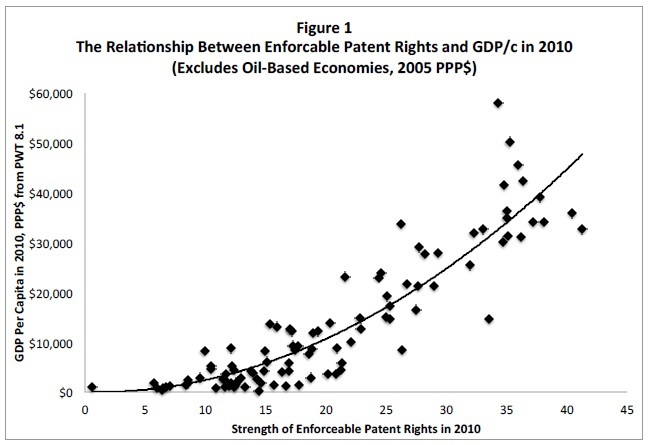
\includegraphics[scale=0.75]{patents_and_gdp.jpg}
\end{center}
\caption{Veza između striktnosti očuvanja patenata zemalja i njihovog bruto domaćeg proizvoda.}
\label{fig:pat_gdp}
\end{figure}

\subsection{Moralni aspekt}
\label{subsec:morala_sam}

\section{Sprovođenje u Srbiji}
\label{sec:srb}

\section{Zaključak}
\label{sec:zakljucak}

Ovde pišem zaključak. 
Ovde pišem zaključak. 
Ovde pišem zaključak. 
Ovde pišem zaključak. 
Ovde pišem zaključak. 
Ovde pišem zaključak. 
Ovde pišem zaključak. 
Ovde pišem zaključak. 
Ovde pišem zaključak. 
Ovde pišem zaključak. 
Ovde pišem zaključak. 
Ovde pišem zaključak. 


\addcontentsline{toc}{section}{Literatura}
\appendix
\bibliography{seminarski} 
\bibliographystyle{plain}

\appendix
\section{Dodatak}
Ovde pišem dodatne stvari, ukoliko za time ima potrebe.
Ovde pišem dodatne stvari, ukoliko za time ima potrebe.
Ovde pišem dodatne stvari, ukoliko za time ima potrebe.
Ovde pišem dodatne stvari, ukoliko za time ima potrebe.
Ovde pišem dodatne stvari, ukoliko za time ima potrebe.


\end{document}
